\begin{flushright}
    در این روش اجازه می‌دهیم تا حرکت به اصطلاح "بد" انجام شود اما در مرور زمان تعداد این حرکات و تاثیرشان را کاهی می‌دهیم.
    در واقع فرض کنید که یک توپ را از بالای تپه‌ای به حرکت در می‌آوریم.
    این توپ ممکن است قبل از رسیدن به min global در یک min local متوقف شود.
    در این صورت با ایزاد یک زمین‌لرزه در یک بازه می‌توانیم از متوقف شدن توپ در min local جلوگیری کنیم.
    \begin{figure}[H]
        \centering
        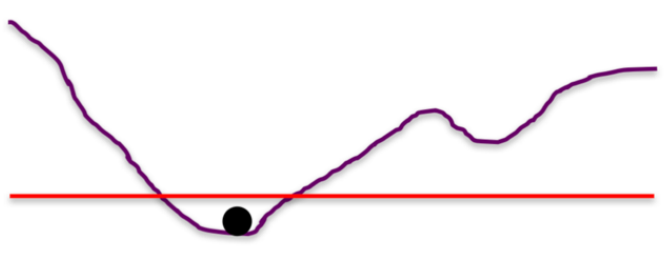
\includegraphics[width=0.5\textwidth]{source/ball.png}
        \label{fig:ball}
    \end{figure}

    همانطور که از اسم این روش مشخص است، الگوریتم برگرفته از یک فرآیند فیزیکی است که در آن با کاهش تدریجی دما، مولکول ها طوری در کنار هم قرار می‌گیرند که ذرات ماده به حالت کریستالی درآیند.
    در این روش اگر دما را با پارامتر T نشان دهیم، این متغیر در گذر زمان کاهش می‌یابد.

    شکل زیر پیاده‌سازی این الگوریتم را نشان می‌دهد.

    \begin{figure}[H]
        \centering
        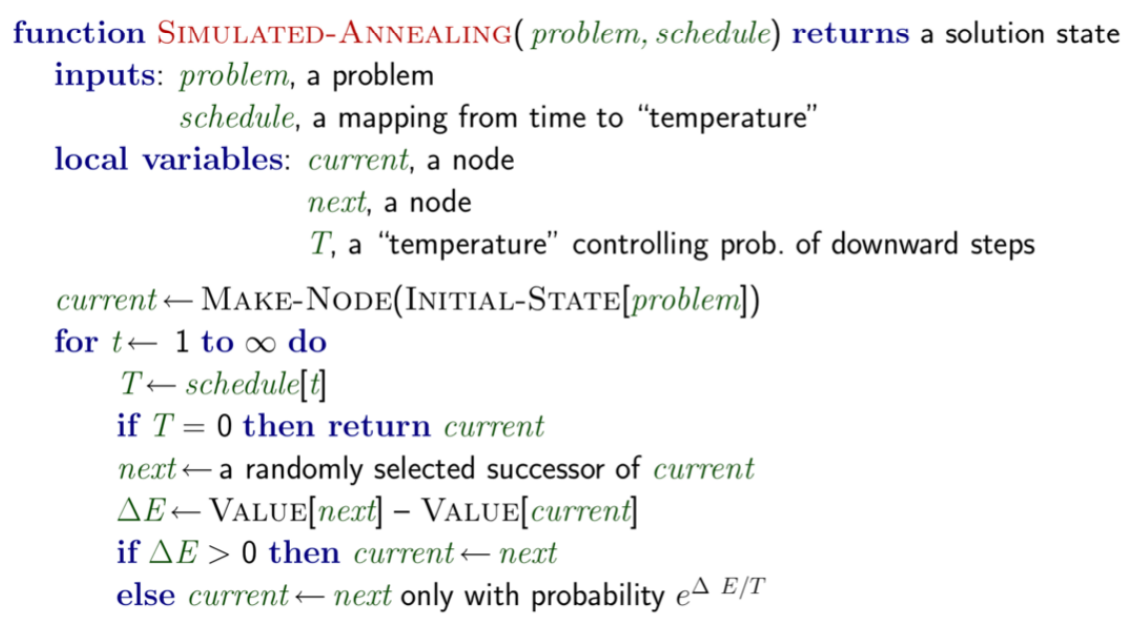
\includegraphics[width=\textwidth]{source/simulated-annealing.png}
        \label{fig:simulated-annealing}
    \end{figure}

    همانطور که می‌بینید، اگر مقدار انتخابی از موقعیت فعلی مقدار بدتری باشد، الگوریتم در گذر زمان به احتمال کمتری این مقدار را به عنوان موقعیت بعدی انتخاب می‌کند.
    نمودار زیر نیزی این امر را تایید می‌کند.
    \begin{figure}[H]
        \centering
        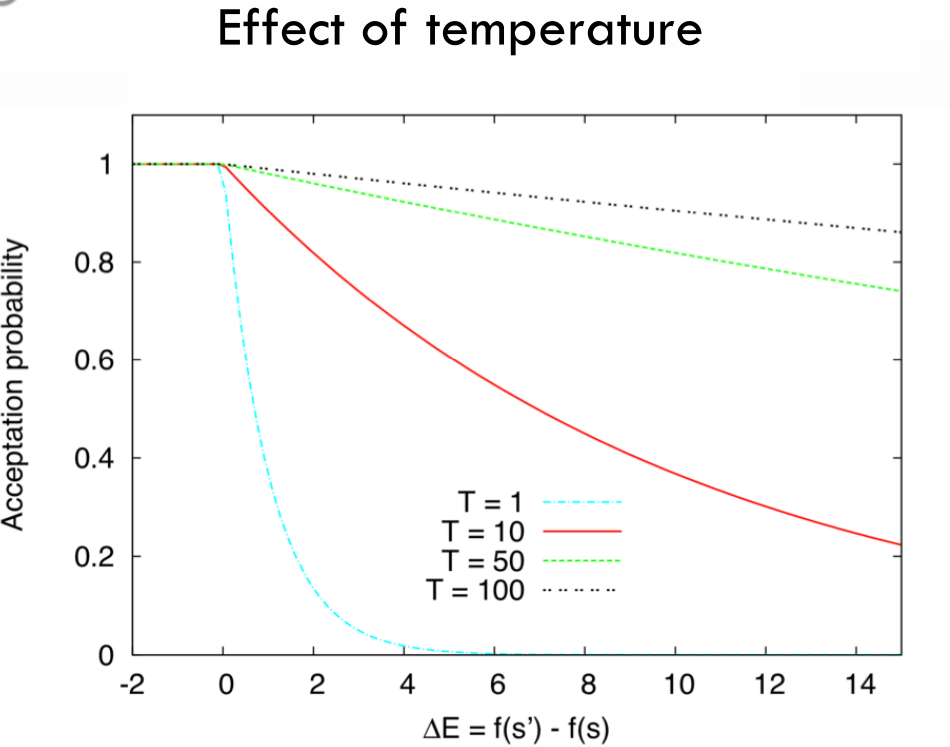
\includegraphics[width=0.7\textwidth]{source/temp-effect.png}
        \label{fig:temp-effect}
    \end{figure}

    می‌توان نشان داد که پارامتر T با شیبی کمتر مساوی $C/log(n)$ کاهش می‌یابد.
\end{flushright}
